\begin{table*}
    \centering
    \begin{tabular}{cc|c|c|c}
       \toprule
        Formula & SrTiO$_3$ & GdFeO$_3$ & BaTiO$_3$ & FeTiO$_3$ \\
        GS TF & .95 & 0.8 & 1.06 & 0.7 \\
        \midrule
\begin{tikzpicture}
  \matrix [label=above:Structures, draw, fill=white, anchor=north east] at (0,0.0) {
    \filldraw[Sr_color] (0,-0.2) circle (0.1cm); & \node {Strontium}; \\
    \filldraw[Ba_color] (0,-0.2) circle (0.1cm); & \node {Barium}; \\
    \filldraw[Gd_color] (0,-0.2) circle (0.1cm); & \node {Gadolinium}; \\
    \filldraw[Ti_color] (0,-0.2) circle (0.1cm); & \node {Titanium}; \\
    \filldraw[Fe_color] (0,-0.2) circle (0.1cm); & \node {Iron}; \\
    \filldraw[O_color] (0,-0.2) circle (0.1cm); & \node {Oxygen}; \\
  };
\end{tikzpicture} & \raisebox{\imageheightoffest\height}{\includegraphics[clip, trim=0cm 0cm 0cm 0cm, width=\imagewidth\linewidth]{figure_images/SrTiO3_crystal.png}} & \raisebox{\imageheightoffest\height}{\includegraphics[clip, trim=0cm 0cm 0cm 0cm, width=\imagewidth\linewidth]{figure_images/GdFeO3_crystal.png}} &\raisebox{\imageheightoffest\height}{\includegraphics[clip, trim=0cm 0cm 0cm 0cm, width=\imagewidth\linewidth]{figure_images/BaTiO3_crystal.png}} & \raisebox{\imageheightoffest\height}{\includegraphics[clip, trim=0cm 0cm 0cm 0cm, width=\imagewidth\linewidth]{figure_images/FeTiO3_crystal.png}} \\

        Graph Nodes
& \raisebox{-.4\height}{\includegraphics[clip, trim=0cm 0cm 0cm 2cm, width=\imagewidth\linewidth]{figure_images/SrTiO3_nodes.png}} & \raisebox{-.4\height}{\includegraphics[clip, trim=0cm 0cm 0cm 2cm, width=\imagewidth\linewidth]{figure_images/GdFeO3_nodes.png}} & \raisebox{-.4\height}{\includegraphics[clip, trim=0cm 0cm 0cm 2cm, width=\imagewidth\linewidth]{figure_images/BaTiO3_nodes.png}} & \raisebox{-.4\height}{\includegraphics[clip, trim=0cm 0cm 0cm 2cm, width=\imagewidth\linewidth]{figure_images/TiFeO3_nodes.png}} \\

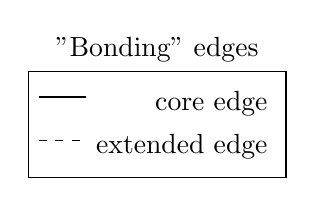
\begin{tikzpicture}
  \matrix [label=above:"Bonding" edges,draw, fill=white, anchor=north east] at (0,0) {
    \draw[black, thick] (0,-0.2) -- (0.6,-0.2); & \node {core edge}; \\
    \draw[black, dashed] (0,-0.2) -- (0.6,-0.2); & \node {extended edge}; \\
  };\end{tikzpicture}& \raisebox{-.4\height}{\includegraphics[clip, trim=0cm 0cm 0cm 2cm, width=\imagewidth\linewidth]{figure_images/SrTiO3_bonds.png}} & 
  \raisebox{-.4\height}{\includegraphics[clip, trim=0cm 0cm 0cm 2cm, width=\imagewidth\linewidth]{figure_images/GdFeO3_bonds.png}} & 
  \raisebox{-.4\height}{\includegraphics[clip, trim=0cm 0cm 0cm 2cm, width=\imagewidth\linewidth]{figure_images/BaTiO3_bonds.png}} & 
  \raisebox{-.4\height}{\includegraphics[clip, trim=0cm 0cm 0cm 2cm, width=\imagewidth\linewidth]{figure_images/TiFeO3_bonds.png}} \\
        
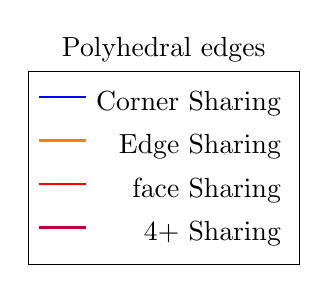
\begin{tikzpicture}
  \matrix [label=above:Polyhedral edges,draw, fill=white, anchor=north east] at (0,0) {
    \draw[blue, thick] (0,-0.2) -- (0.6,-0.2); & \node {Corner Sharing}; \\
    \draw[orange, thick] (0,-0.2) -- (0.6,-0.2); & \node {Edge Sharing}; \\
    \draw[red, thick] (0,-0.2) -- (0.6,-0.2); & \node {face Sharing}; \\
    \draw[purple, thick] (0,-0.2) -- (0.6,-0.2); & \node {4+ Sharing}; \\
  };\end{tikzpicture}&
  \raisebox{-.4\height}{\includegraphics[clip, trim=0cm 0cm 0cm 2cm, width=\imagewidth\linewidth]{figure_images/SrTiO3_poly.png}} & 
  \raisebox{-.4\height}{\includegraphics[clip, trim=0cm 0cm 0cm 2cm, width=\imagewidth\linewidth]{figure_images/GdFeO3_poly.png}}  & 
  \raisebox{-.4\height}{\includegraphics[clip, trim=0cm 0cm 0cm 2cm, width=\imagewidth\linewidth]{figure_images/BaTiO3_poly.png}}  &
  \raisebox{-.4\height}{\includegraphics[clip, trim=0cm 0cm 0cm 2cm, width=\imagewidth\linewidth]{figure_images/TiFeO3_poly.png}}  \\
        \bottomrule
    \end{tabular}
    \begin{tabular}{l|cccc|cccc}
        
        & \multicolumn{4}{c|}{Topology Scores} & \multicolumn{4}{c}{Distortion Scores}\\
        \hline
         & SrTiO$_3$  & LaNiO$_3$  & CaIrO$_3$ & FeTiO$_3$  & SrTiO$_3$  & LaNiO$_3$   & CaIrO$_3$   & FeTiO$_3$ \\
        \hline
        SrTiO$_3$ & - & 0.947 & 0.885 & 0.231 & - & 0.560 & 0.412&  0.321\\
        LaNiO$_3$ & 0.947 & - & 0.925 & 0.242 & 0.560 & - & 0.642 & 0.349\\
        CaIrO$_3$ & 0.885 & 0.925& - & 0.265 & 0.412 & 0.642 & - & 0.441\\
        FeTiO$_3$ & 0.231 & 0.242& 0.265 & - & 0.321 & 0.349& 0.441 & - \\
        \hline
    \end{tabular}
    \captionsetup{justification=centering}
    \caption{Comparison of condensed crystal graphs for four 113 formula ratio materials. a) SrTiO$_3$, a prototypical cubic peroskite. b) GdFeO$_3$, a distorted perovskite. c) BaTiO$_3$, a distorted perovskite. d) FeTiO$_3$, a prototypical ilmenite structure. Graph visualization condenses symmetry equivalent edges and nodes into one for clarity. The table shows the topology and distortion scores between the four compounds. The three perovskite compounds score high in topology score, indicating similar underlying connectivity in the structure. They show various level of distortion, with the two distorted perovskites showing more similar distortions than the cubic perovskite. The ilmenite structure scores poorly on topology will all perovskites, reflecting that it is fundamentally a different structure. While graphs have similar local connectivity, seen in the similarity of Ti-O bonds across graphs, polyhedral edges differ widely between dissimilar structures. The distortion score between fundamentally different structures has little meaning.}
    \label{fig:113_example_fig_and_table_new}
\end{table*}
